%!TEX root=thesis.tex

\chapter{Radio Cross-identification}
\label{cha:passive-learning}
  % In this chapter I'll talk about a machine learning approach to the cross-identification problem (i.e. my pipeline).

  In this chapter, I develop a machine learning approach to the radio cross-identification problem. First, I will discuss different ways to train and use a classifier for the task, in particular framing the cross-identification problem as an object localisation problem. Then, I will discuss the available training data and how I chose to process it. Finally, I will present results against a dataset of expert labels, and compare these results to those found by other methods.

\section{Cross-identification as Binary Classification}
\label{sec:framing-as-classification}
  
  Given a radio object, we want to locate the host galaxy containing the AGN emitting that object. In general, there may be multiple hosts associated with one radio object (such as in Figure \ref{fig:two-hosts}), but we make the assumption that there is only one. This is the same assumption made by Radio Galaxy Zoo \todo{cite:rgz-analysis-github(?)}.

  \begin{figure}[!ht]
    \centering
    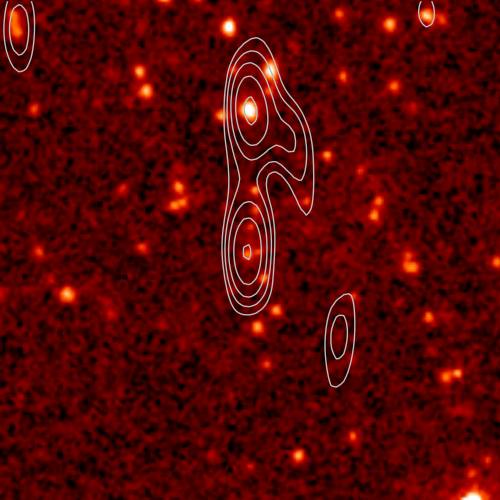
\includegraphics[width=0.5\textwidth]{images/CI0370C1_heatmap+contours.png}
    \caption{A radio object (ARG0003ra1) with two host galaxies. This radio
      object is actually two radio objects that have been incorrectly detected
      as one, and there is one host galaxy for each object.}
    \label{fig:two-hosts}
  \end{figure}

  We can interpret this as an object localisation problem. As input, we have an
  image of the radio sky, and we want to locate a host galaxy in this image. A
  common way to find an object in an image is by using a sliding window. A
  fixed-size image patch centred on each pixel is taken as a feature
  representation of that pixel. This is then used as input to a classification
  model which outputs a probability for each pixel, with higher probabilities
  corresponding to higher likelihood of the object being located at that pixel.
  The pixel with the highest rating is considered the location of the object.
  This approach can be improved by intelligently selecting candidate pixels and
  only testing these. For the cross-identification problem, we can use galaxy
  locations as candidate pixels, with galaxies found in infrared surveys such
  as WISE and SWIRE.

  This approach can be formalised as follows. Consider a set $\mathcal X$ of
  candidate host galaxies, and a radio object $r$ that we want to assign a
  host galaxy. Let $y : \mathcal X \to \{0, 1\}$ represent whether a given $x
  \in \mathcal X$ is the host galaxy associated with $r$. If we assume that a
  radio object has exactly one associated host galaxy, then there exists
  exactly one $x \in \mathcal X$ such that $y(x) = 1$, and for all other $x \in
  \mathcal X$, $y(x) = 0$. The cross-identification task then amounts to
  modelling $p(y(x) = 1 \mid x, r)$. Once this distribution is modelled, the
  host galaxy associated with $r$ is given by
  \begin{equation}
      \label{eq:cross-identification}
      \mbox{host}(r) = \underset{x}{\mbox{argmax}}\ p(y(x) = 1 \mid x, r).
  \end{equation}

  Ideally, $\mathcal X$ is the set of all galaxies. This is clearly
  intractable, so as an approximation we use a catalogue of infrared objects
  near the radio object of interest, taken from an infrared survey. We also
  make the assumption that the host galaxy is within $1'$ of the radio object
  --- while this doesn't hold in general, systems larger than $1'$ are rare and
  require human insight to discover \citep{banfield16}.

\section{Data Sources}
\label{sec:data}

  To learn the cross-identification distribution (Equation \ref{eq:cross-identification}), we need a set of radio objects, a set of candidate host galaxies, and a set of radio objects and their associated host galaxies. For this, I have chosen 

  \subsection{Radio Data}
  \label{ssec:radio-data}

    Radio objects for cross-identification were taken from the ATLAS survey \citep{franzen15}.

  \subsection{}

\section{Choosing a Binary Classifier}
\label{sec:binary-classifier}

\section{Results}
\label{sec:passive-results}
